\documentclass[10pt,a4paper]{article}
\usepackage[utf8]{inputenc}
\usepackage{amsmath}
\usepackage{amsfonts}
\usepackage{amssymb}
\usepackage{graphicx}
\usepackage{float}
\usepackage{breqn}
\usepackage{natbib}
\usepackage[spaces,hyphens]{url}
\usepackage[colorlinks,allcolors=blue]{hyperref} 

\def\sinc{\mathop{\rm sinc}\nolimits}

\title{Polarization in a LISA verification binary}

\begin{document}

\maketitle

\section{GW signal from a binary}

According to general relativity, gravitational waves have two
polarizations $h_+(t)$ and $h_\times(t)$.  The time dependence can be
anything, but here we are interested in the case where both have the
same period but are out of phase.  A GW interferometer measures a
time dependent strain
\begin{equation}
  \frac{\delta L}L = 
  \left( h_+ \, F_+ + h_\times \, F_\times \right)
\end{equation}
where $F_+$ and $F_\times$ are the response functions of the
instrument.  If the signal is periodic, the amplitude of the measured
signal will be
\begin{equation}
  \left(|h_+ \, F_+|^2 + |h_\times \, F_\times|^2 \right)^{1/2}
\end{equation}
Let us now consider what $h_+,h_\times,F_+,F_\times$ depend on.

A binary emits GW as
\begin{equation}
\begin{pmatrix}
  h_+\\h_\times
\end{pmatrix}
= \frac{8GE}{c^4 D}
\begin{pmatrix}
  \frac12(1+\cos^2\iota) \\
  i\cos\iota
\end{pmatrix}
\exp(i\omega t)
\end{equation}
where $E$ is the orbital energy and $\omega$ is twice the orbital
frequency.

\begin{figure}[h]
\centering
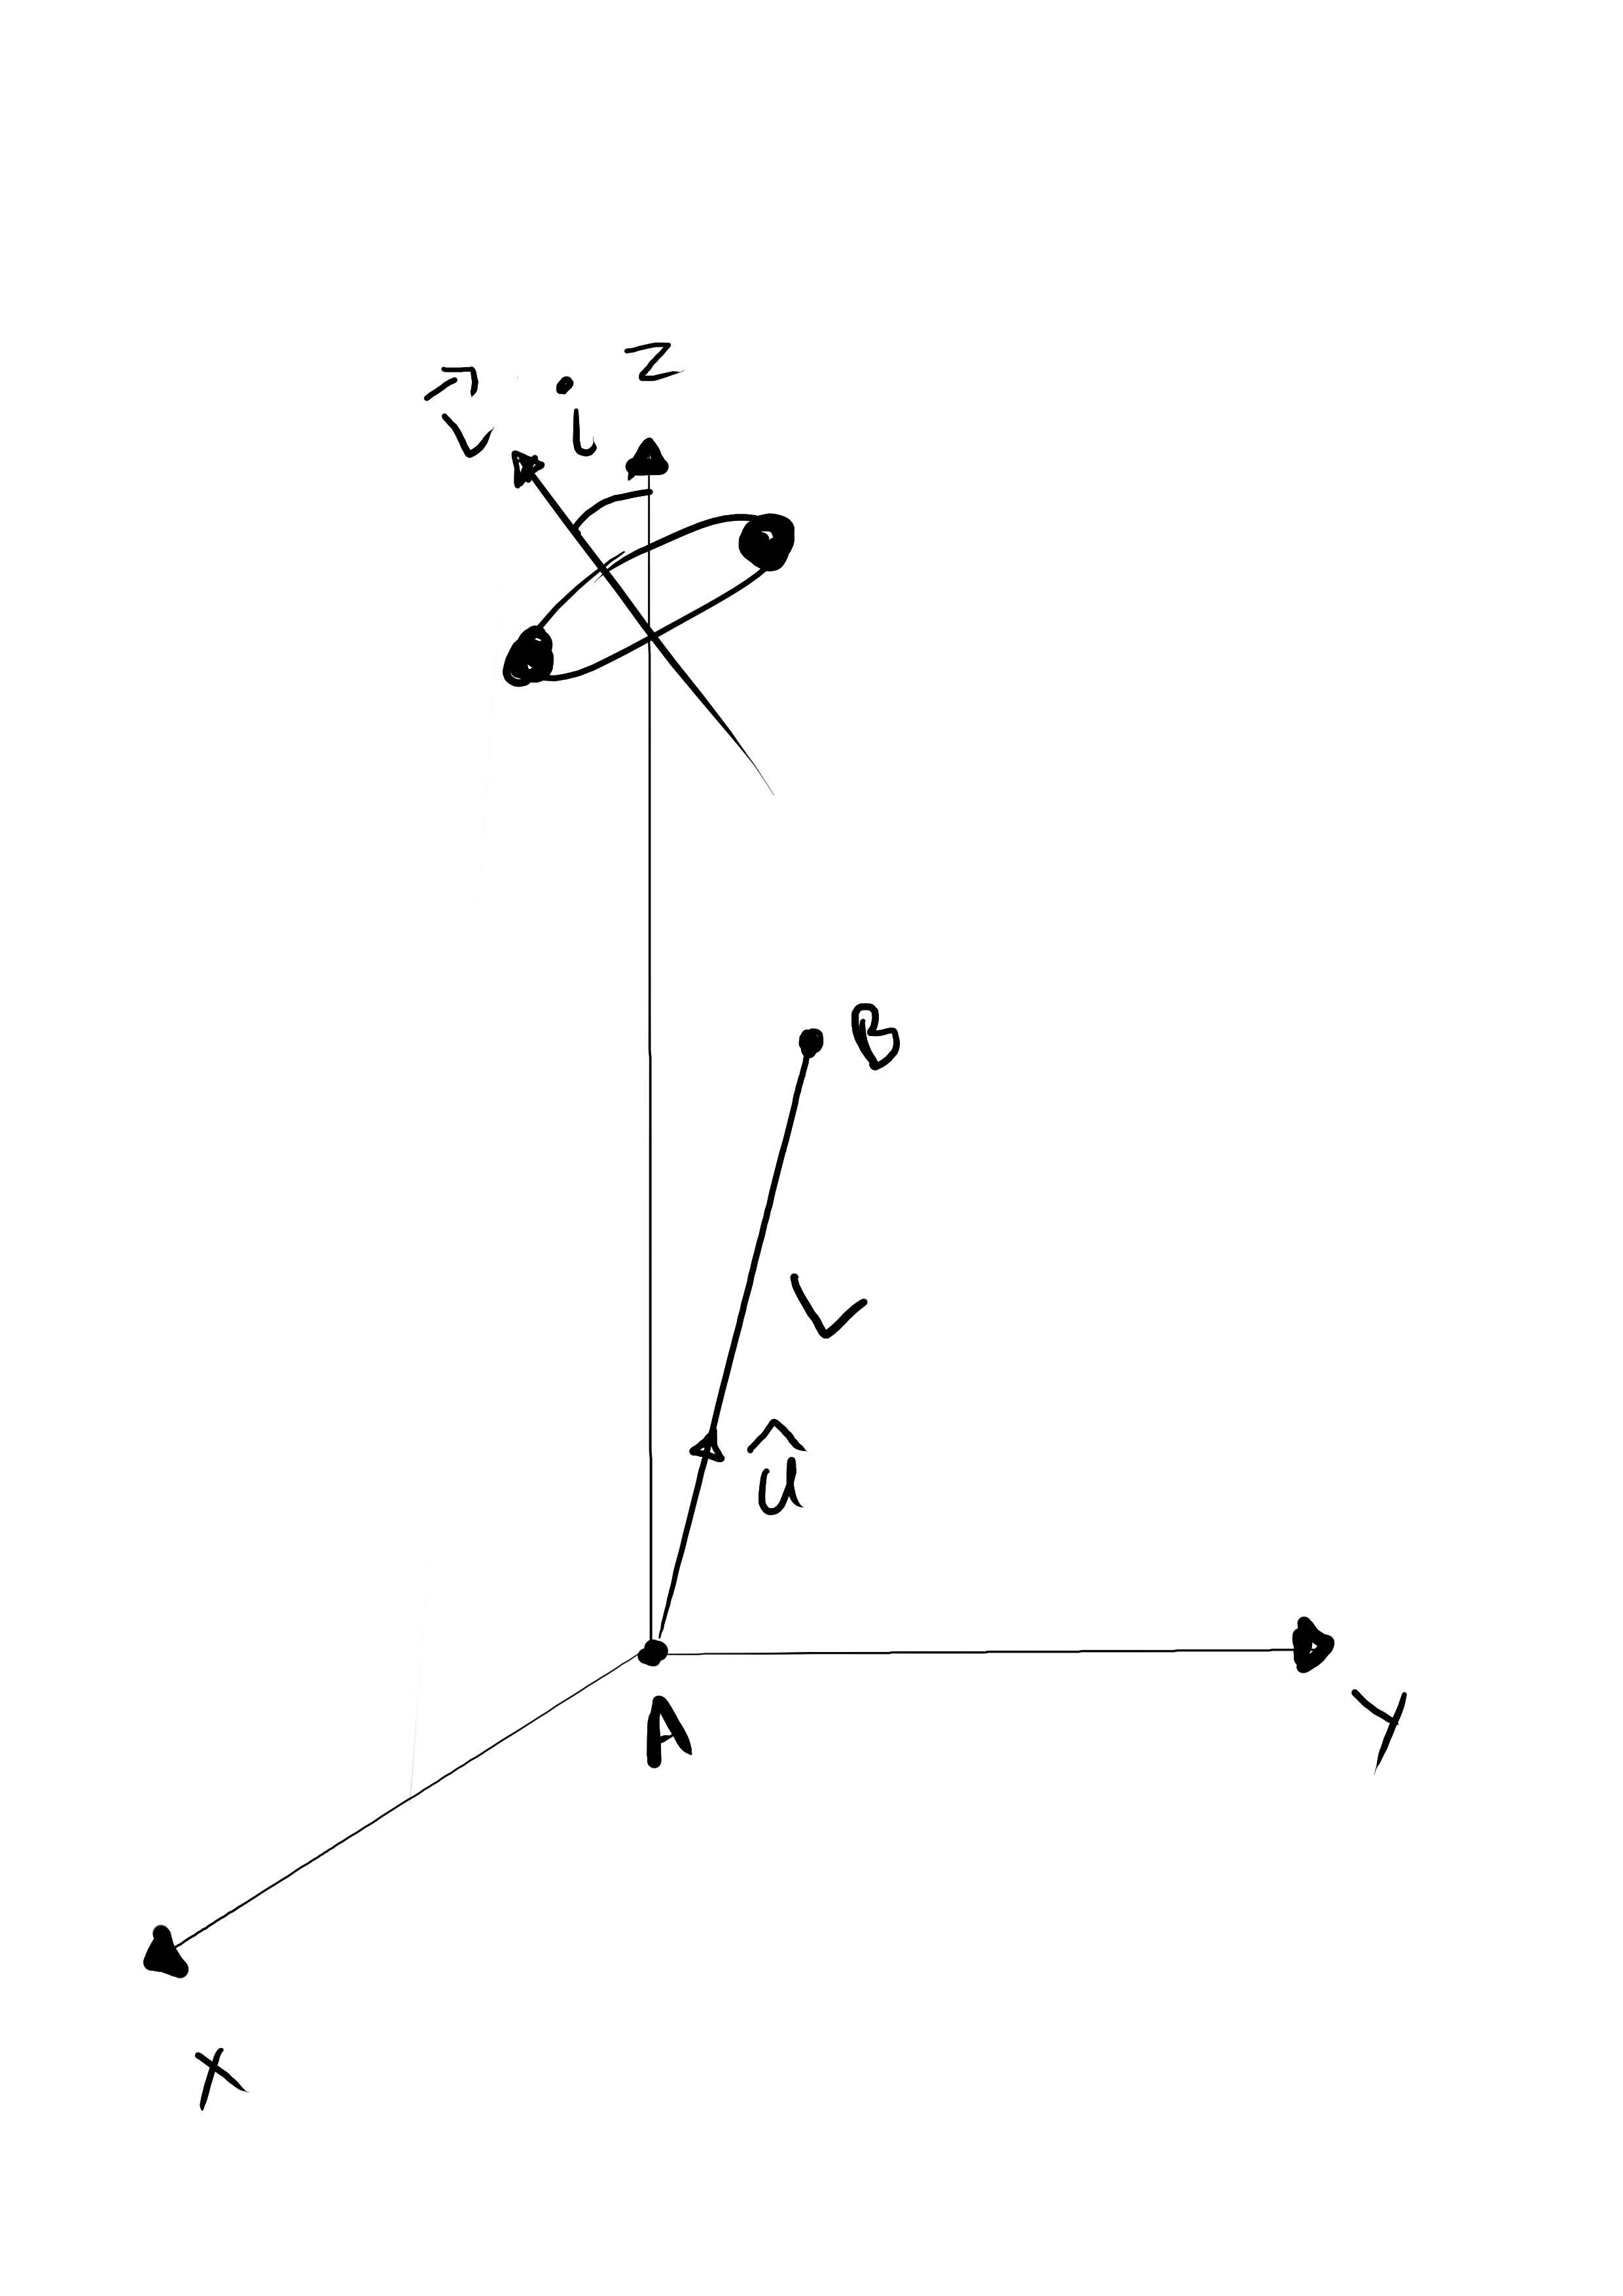
\includegraphics[scale=0.25]{../Figures/diagram1.jpg}
\caption{The one arm arrangement with the source on the $z$-axis with
  angle of inclination $\iota$ and the arm in the $x$-$z$
  plane.\label{fig:binary}}
\end{figure}

We now consider the geometry in Figure~\ref{fig:binary}.  We take the
$z$ axis to be the line of sight.  The binary is on a circular orbit
inclined at angle $\iota$ to the line of sight ($\iota=0$ is face-on)
and the inclination has a position angle $\psi$.  This last angle
applies a rotation to $h_+$ and $h_\times$ and is the polarization
angle.  A GW interferometer may have two perpendicular arms (LIGO) or
three arms in a triangle (LISA).  For our purposes, however, it is
enough to consider a single arm.  We take this arm to be in the
$x$-$z$ plane and at angle $\theta$ with respect to the line of sight.
The spacecraft at the origin sends a series of photons while the weak
plane gravitational wave passes through space in the $+z$ direction.
The metric in the transverse-traceless gauge is
\begin{equation}
\begin{aligned}
ds^2 &= -c^2 dt^2 + dz^2 \\
&+ (1 + h_+\cos2\psi + h_\times\sin2\psi) \, dx^2 \\
&+ (1 - h_+\cos2\psi - h_\times\sin2\psi) \, dy^2 \\
&- 2(h_+\sin2\psi - h_\times\cos2\psi) \, dx\,dy
\end{aligned}
\end{equation}
Using this metric we can
compute the round trip of a photon along an arm of length $L$ and 
back again.  Extending the derivation given in \cite{cornish} for
one polarization to two polarizations, we get
\begin{equation}
\begin{pmatrix}
  F_+\\F_\times
\end{pmatrix}
= {\textstyle\frac12} \sin^2\theta 
\begin{pmatrix}
  \cos2\psi\\
  \sin2\psi
\end{pmatrix}
\tau(\omega,\theta,L) 
\end{equation}
The last factor is
\begin{equation}
\begin{aligned}
  \tau(\omega,\theta,L) \equiv
  &\sinc(\alpha(1-\cos\theta))\,\exp(-i\alpha(3+\cos\theta)) \, + \\
  &\sinc(\alpha(1+\cos\theta))\,\exp(-i\alpha(1+\cos\theta))
\end{aligned}  
\end{equation}
where $\alpha\equiv(\omega L)/(2c)$.  In the low frequency limit
$\tau\to1$.  The measured strain is then
\begin{equation}
\frac{2GE}{c^4 D} \sin^2\theta
  \left((1+\cos^2\iota)^2 \cos^2 2\psi + 4\cos^2\iota \sin^2 2\psi\right)^{1/2}
\end{equation}
which as we see depends on the angle of orientation of the arm
$\theta$ with respect to the line of sight, the angle of inclination
of the orbit $\iota$, and the polarization angle $\psi$.
Figure~\ref{fig:resporient} illustrates the dependence on $\iota$ and
$\psi$.

\begin{figure}[!h]
\centering
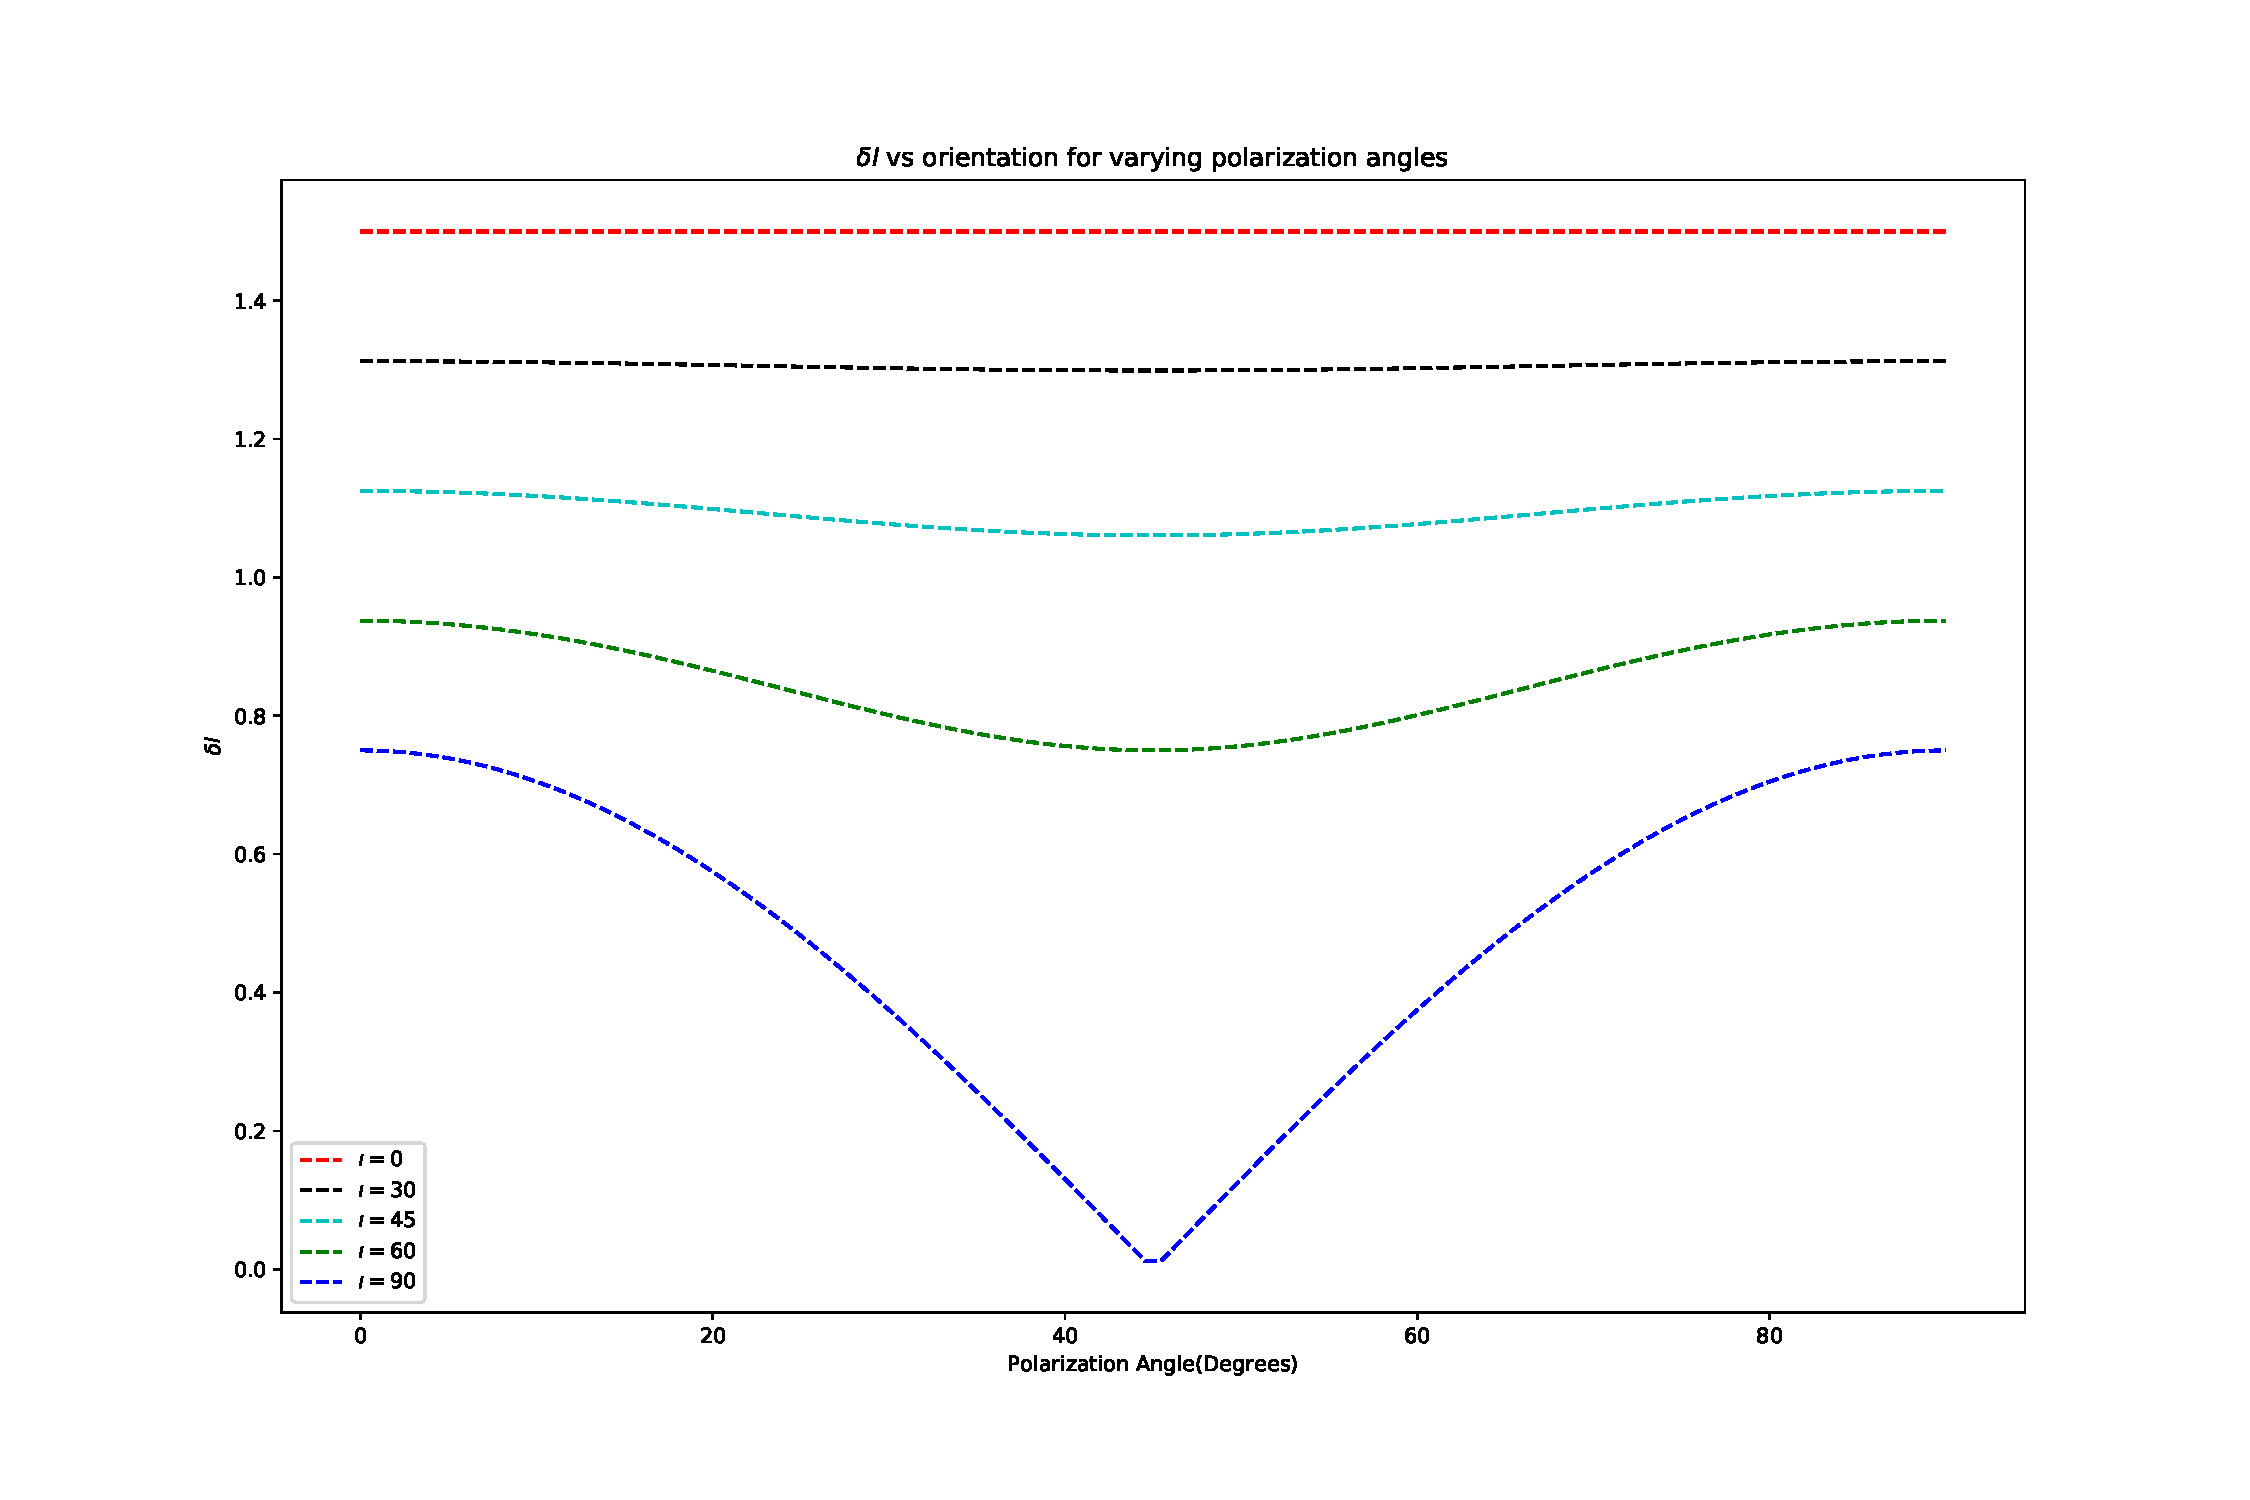
\includegraphics[scale=0.3]{../Figures/responsevsorientationofbinary.pdf}
\caption{The response $\delta l/L$ varying with the polarization
  angle $\psi$ for various inclination angle.\label{fig:resporient}}
\end{figure}

There are several other ways of expressing the strain.  \cite{cornish}
in their eq.~(8) give a coordinate-free formula.  \cite{ACST}
consider a LIGO-like system with the arms along the $x$ and $y$ axes.
\cite{cutler} considers a pair of LISA arms.
 
\newpage
\section{LISA Verification Binaries}

The Laser Interferometer Space Antenna(LISA) will be the first gravitational wave observatory in space. LISA will be operating in the low frequency part of the gravitational wave spectrum($10^4$--1 Hz). In this range, we expect to observe lots of ultracompact binaries with orbital periods shorter than few hours. Out of these UCBs, AM CVn type binaries are of particular interest. Due to therir strong GW signals, they are guaranteed to be  detetcted on LISA band. These are termed `verification binaries'.

We are interested in providing an independent measurement of $\psi$ and if possible $\iota$.

\begin{figure}[ht]
\centering
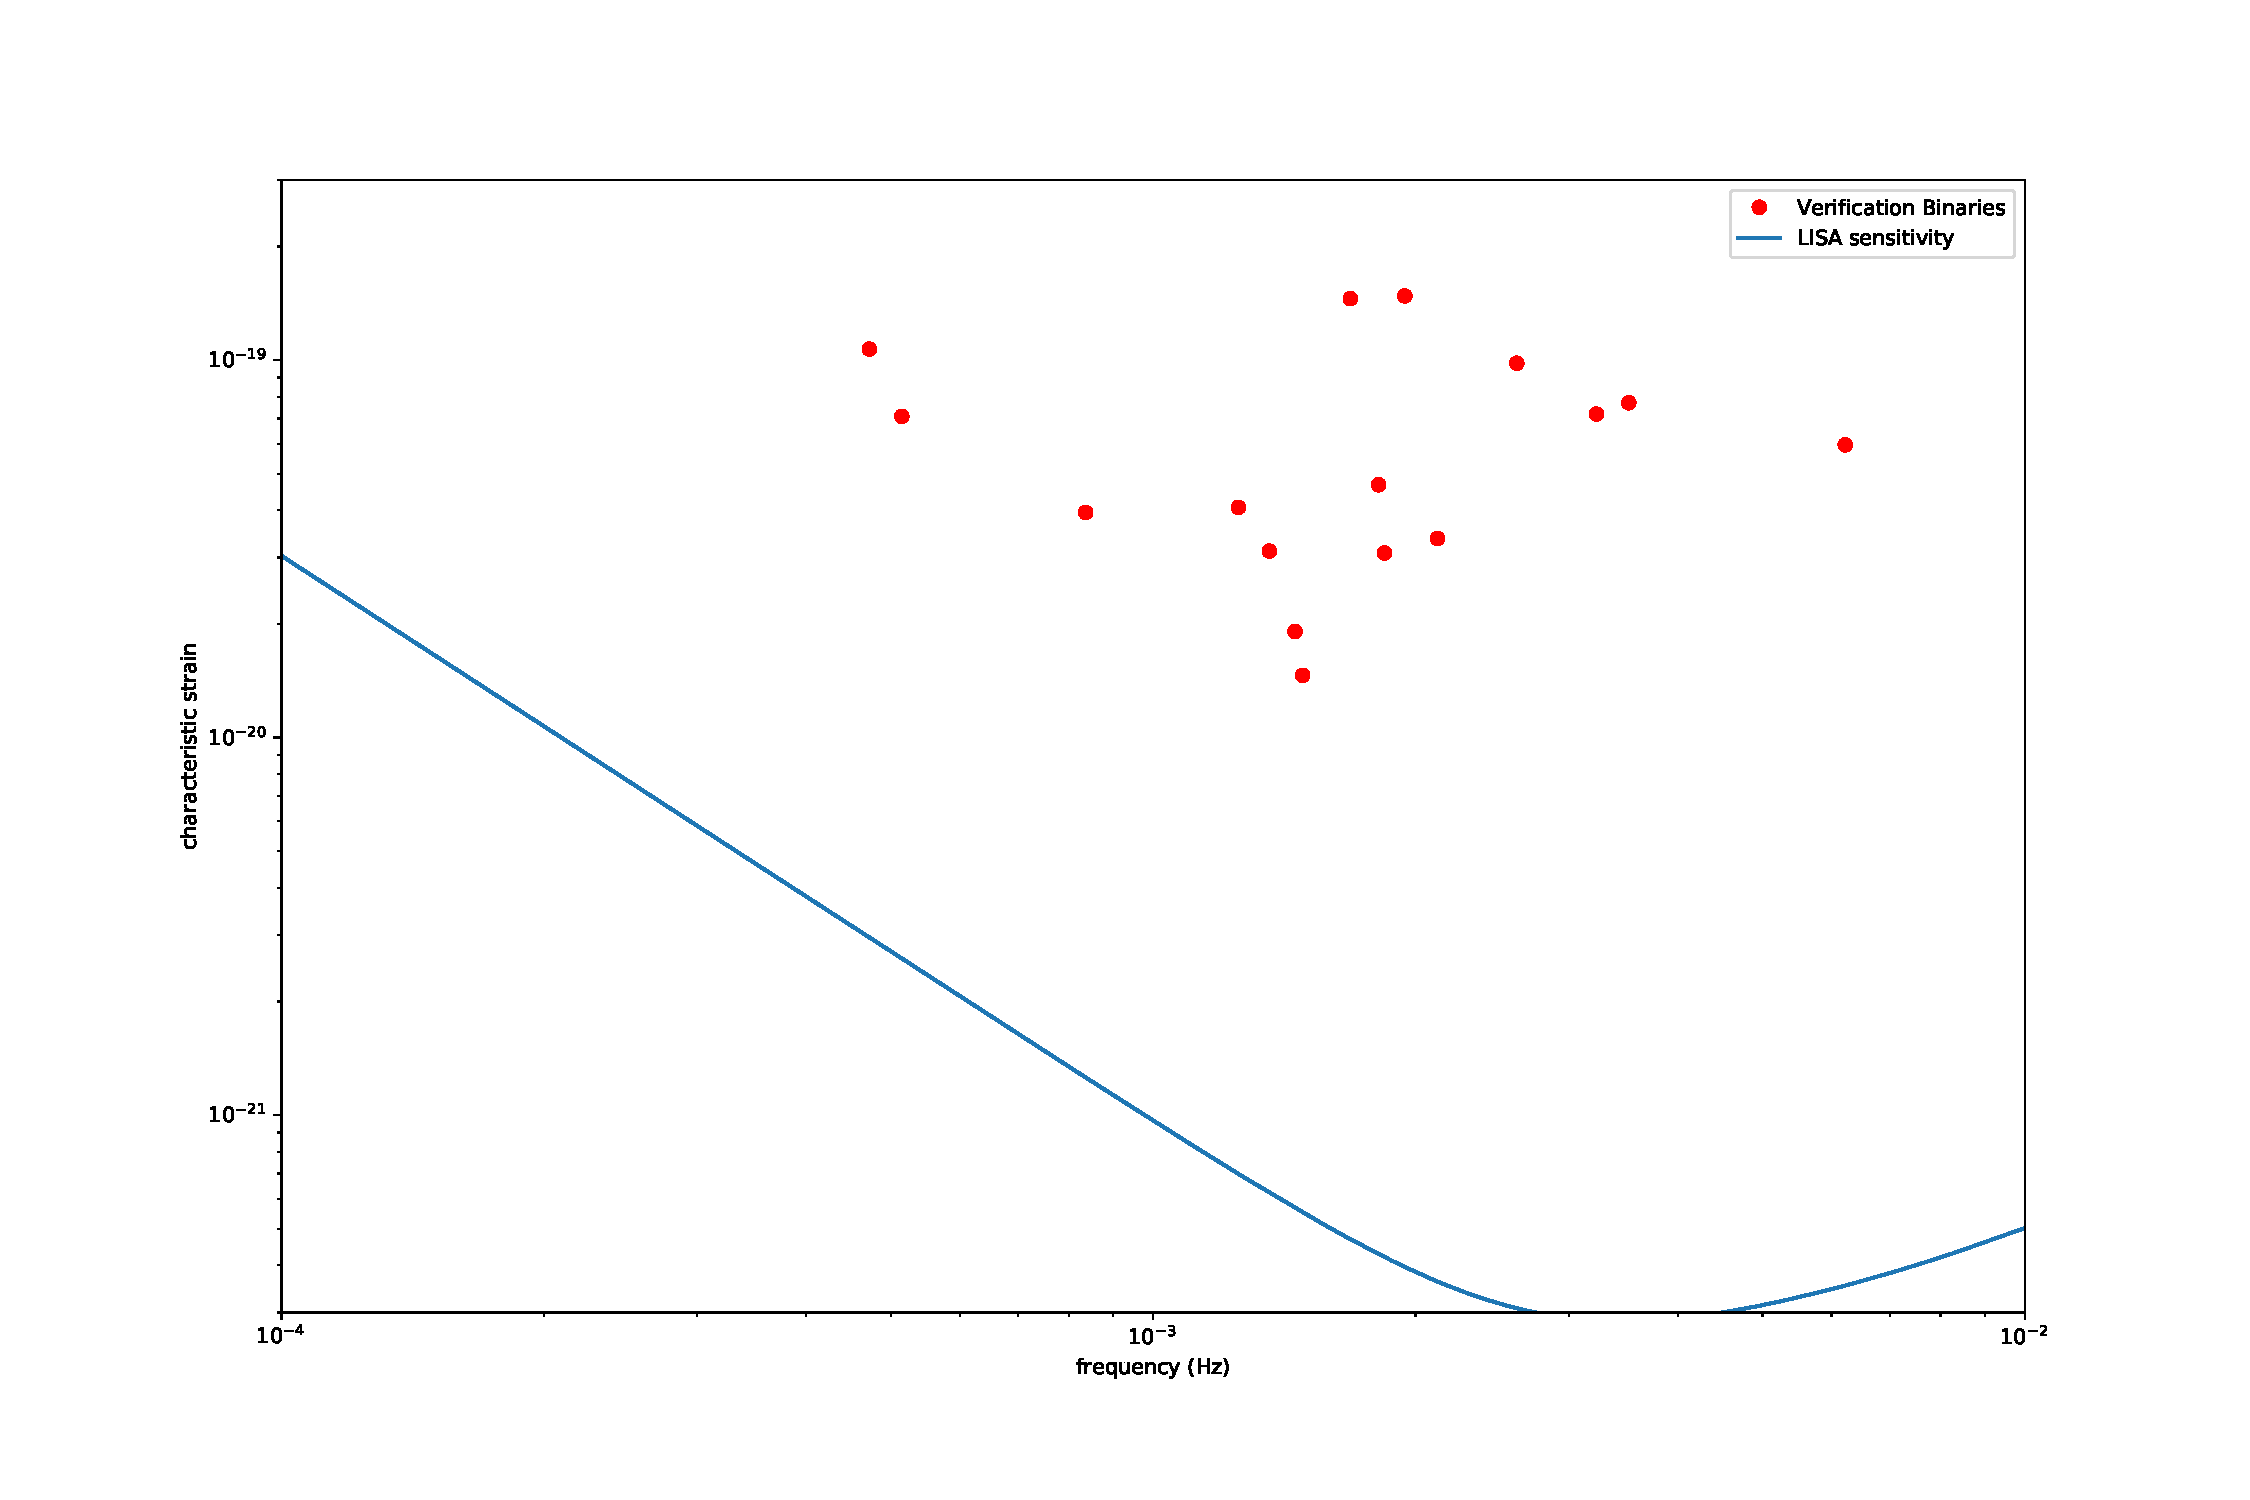
\includegraphics[scale=0.25]{../Figures/strain_verific_binary.pdf}
\caption{The calculated strains due to LISA verification binaries and the sensitivity curve of LISA}
\end{figure}

\section{HP Lib Verfication Binary}

The most promising system appears to be the AM CVn binary HP Lib. The binary consist of a high-mass white dwarf and a low-mass star (brown dwarf).

The mass of the binaries are found from the lightcurves. \cite{Patterson} also gives the masses M1 and M2. The inclination of the system is reported in \cite{Roelofs}


Also, the radius of the secondary can be found using the reation mentioned in \citep{Patterson}

\begin{equation}
R_{zs} = 0.0155 \ m_2^{-0.212}
\end{equation}
For $m_2 = 0.048$, $R_2 = 0.030$ in solar units.

\begin{table}[H]
\centering
\begin{tabular}{|c|c|c|c|c|}
\hline 
\rule[-1ex]{0pt}{2.5ex} Source & $m_1$($M_{\odot}$) & $m_2$($M_{\odot}$) & $P_{\rm orb}$(sec) &i (degrees) \\ 
\hline 
\rule[-1ex]{0pt}{2.5ex} HP Lib & 0.49--0.80 & 0.048--0.08 & 1102.70 & 26-34\\ 
\hline 
\end{tabular}
\caption{The estimated values of mass and time period of HP Lib}
\label{table1}
\end{table}

Table [\ref{table1}] lists the estimated values as mentioned in paper \cite{Roelofs}\\



Consider the verification binary HP Lib with masses $m_1$ and $m_2$
and period $P$. We can find the fraction of light received by the
brown dwarf $m_2$ in the following way:

The flux from mass $m_1$ obeys the inverse square law. Assuming a
luminosity $L$, the flux at a distance $d$ is given by $L/4 \pi
d^2$. The cross section area for brown dwarf is $\pi R^2$.

Therefore, the total flux received is:
\begin{equation}
\frac{L}{4 \pi d^2} \ \pi R^2 = \frac{L}{4} \ \left(\frac{R}{d}\right)^2
\end{equation}
where $R$ is the radius of the brown dwarf and $d$ is the separation.
From Kepler's third law, using the Earth's orbit as a reference, we have
\begin{equation}
  \frac{1}{4} \left(\frac{R}{\rm 1\,au}\right)^2
  \left(\frac{M}{M_{\odot}}\right)^{-2/3}
  \left(\frac{P}{P_{\oplus}}\right)^{-4/3}
\end{equation}
For a first estimate, we can take $R = 0.03R_\odot$ or $R/c \approx
0.07$ which if we substitute above we estimate the fraction of light
received is $\approx 0.0064$.

From the light curves (Fig.4) of \citep{Patterson}, the apparent magnitude in the V band ($M_V$) is $\approx 13.7$.

\def\pasp{PASP}

\bibliographystyle{aa}
\bibliography{refs.bib}

\end{document}

\begin{thebibliography}{9}

\bibitem{cornish}				\url{https://arxiv.org/pdf/gr-qc/0103075.pdf}

\bibitem{whelan} \url{https://dcc.ligo.org/public/0106/T1300666/003/Whelan_notes.pdf}
\end{thebibliography}






\begin{multline}
ds^2 = - c^2 dt^2 + (1+ h_+ \cos 2\psi + h_x \sin 2 \psi) d x^2 +(1- h_+ \cos 2\psi - h_x \sin 2 \psi) d y^2 \\
 - 2(h_+ \sin 2 \psi - h_x \cos 2 \psi) dx dy + dz^2
\end{multline}

\begin{equation}
\label{resp}
\delta l(t_2) = \frac{L \sin^2 \theta}{2} \ \tau(\cos \theta,f) \left[ h_{+}(t_2) \cos 2\psi + h_{x}(t_2) \sin 2\psi \right]
\end{equation}

$\tau$ is the transfer function as defined in eq(7) of \cite{cornish}

Now from we consider the plus and cross polarisation amplitudes of a binary black hole with an angle of inclination $i$ with the line of sight $\hat{z}$ (3.27a and 3.27b) \cite{whelan}. 

Substituting the $h_{+}$ and $h_{x}$ expressions, eq [\ref{resp}] becomes,
\begin{align}
\delta l&=\frac{A(t) L \sin^2 \theta \tau(\cos \theta,f)}{2d} \left[\frac{1+\cos^2 i}{2} \ \cos 2\psi \ \cos \Phi(t) + \cos i \ \sin 2\psi \ \sin \Phi(t)\right]\\
&=\frac{A(t) L \sin^2 \theta \tau(\cos \theta,f)}{2d} \left( \sqrt{ \frac{(1+\cos^2 i)^2}{4} \cos^2 2\psi  + \cos^2 i \sin^2 2\psi} \right)\cos(\Phi(t)-\Psi)
\end{align}

Where $\Phi(t) = 2 \pi f t + \Phi_0$.

For a general location of the binary ($\hat{\Omega}$) specified by $\theta_s,\omega$ in spherical coordinate system, we can derive the antenna beam patterns\cite{whelan}.T

\begin{align*}
F_{+}(\theta_s,\phi,\psi,i)&=\frac{(1+\cos^2 i)}{2} \left[\frac{1}{2}(1+ \cos^2 \theta_s) \cos2\phi \cos\psi - \cos\theta_s \sin2\phi \sin2\psi \right]\\
F_{\times}(\theta_s,\phi,\psi,i)&=\cos i \left[\frac{1}{2}(1+ \cos^2 \theta_s) \cos2\phi \cos\psi + \cos\theta \sin2\phi \cos2\psi \right]\\ 
\end{align*}

If we put back $\theta_s=0$ and $\phi=0$ in these equations we get back the responses in eq [4].

We can form an interferometer by introducing a third spacecraft at a distance L from the corner spacecraft and subrating the outputs of the two arms \cite{cornish} to get the total strain.


\begin{align}
s(\hat{\Omega},f,\textbf{x},t)&=\frac{\delta l_u (t) - \delta l_v (t)}{l}\\
&=\textbf{D}(\hat{\Omega},f) : h(\hat{\Omega},f,\textbf{x},t)
\end{align}

where $$D(\hat{\Omega},f) = \frac{1}{2}\left((u \otimes u) \tau - (v \otimes v) \tau \right)$$

is the detector response tensor. \textbf{u} and \textbf{v} are the unit vectors representing the direction of each interferometer arm. $\hat{\Omega}$ is the direction of propegation of the wave. We can use the orientation of LISA arms and compute the detetctor response functions $F_{+}$ and $F_{\times}$.






Consider the verification binary HP Lib with masses $m_1$ and $m_2$ and period P \ref{1}. We can find the fraction of light recieved by the brown dwarf $m_2$ in the following way:

The flux from mass $m1$ obeys the inverse square law. Assuming a luminosity L, the flux at a distance d is given by $L/4 \pi d^2$. The cross section area for brown dwarf is $\pi R^2$.


Therefore, the total flux recieved is: $$\frac{L}{4 \pi d^2} \ \pi R^2 = \frac{L}{4} \ \left(\frac{R}{d}\right)^2 $$ where R is the radius of the brown dwarf and d is the seperation.

We can estimate d from the time period of the orbit. We know from Kepler's 3rd law that, $T^2 = \frac{4 \pi^{2}}{G (m_1 + m_2)} d^3$. We will denote $M=m_1 + m_2$

\begin{align*}
\frac{d}{c}&=\left(\frac{GM}{c^3}\right)^{1/3} \frac{T^{2/3}}{(4 \pi^{2})^{1/3}}\\
&=\frac{\left(\frac{GM}{c^3}\right)^{1/3}}{\left(\frac{GM_{\odot}}{c^3}\right)^{1/3}} \frac{T^{2/3}}{(4\pi^2)^{1/3}} (5 \times 10^{-6})^{1/3}
\end{align*}

Now the fraction of the light recieved is,

\begin{equation}
\frac{1}{4} \left(\frac{R}{c}\right)^2 \left(\frac{M}{M_{\odot}}\right)^{-2/3} \frac{T^{-4/3}}{(4 \pi^2)^{-2/3}} (5 \times 10^{-6})^{-2/3}
\end{equation}

For the first estimate, we can take $R/c \approx 0.07$ which if we subtitute above give an estimate of the light received to be 0.01315

----



LISA's response function can be calculated by imagining it as a two arm Michelson interferometer. We first derive the response of a single arm and then cross correlate with the other to measure the total strain.

Consider two LISA spacecraft, one ar the origin and another at a distance L away from it.  We choose the coordinate axes such that the spacecrafts lie in the x-z plane. The vector  $ \textbf{u} = \hat{x} \ \sin \theta + \hat{z} \ \cos \theta$ describes the single arm here.

In general the strain $h(t)$ can be written as a linear combination of $h_{+}(t)$ and $h_{\times}(t)$.

\begin{equation}
h(t) = F_{+}(\theta_s,\phi_s,\psi_s) h_{+}(t) + F_{\times}(\theta_s,\phi_s,\psi_s)
\end{equation}

We can rewrite the signal from the binary in the conventional amplitude-and-phase form.

\begin{equation}
h(t) = -A(t) \cos[2\Phi(t) +\varphi]
\end{equation}

where $A(t)$ is given by



\begin{equation}
A(t) = \frac{2 G \mu M}{c^4 a D}\left([1+(\hat{\textbf{L}} \cdot \hat{\textbf{N}})^2]^2 F_{+}^2(\theta_s,\phi_s,\psi_s) + 4[\hat{\textbf{L}} \cdot \hat{\textbf{N}}]^2 F_{\times}^2(\theta_s,\phi_s,\psi_s) \right)^{\frac{1}{2}}
\end{equation}

Where $\hat{\textbf{L}}$ and $\hat{\textbf{N}}$ are the unit vectors along the angular momentum of the binary and the one along the line of sight in the detector frame respectively. $\phi(t)$ represents the phase. 
Also, $\hat{\textbf{L}} \cdot \hat{\textbf{N}} = \cos \ \iota$ where $\iota$ is the inclination of the binary. These are defined in the Figure \ref{fig:directions} from \citep{ACST}.\\ 

The detector beam patterns $F_{+}$ and $F_{\times}$ depend on the source direction and the  polarization angle $\psi$.\citep{cutler}. The polarization angle $\psi$ is the angle from the principal + direction ($\hat{\textbf{N}} \times \hat{\textbf{L}}$) , clockwise in the plane of sky to the azimuth($\hat{\textbf{N}} \times (\hat{\textbf{N}} \times \hat{\textbf{z}})$). The polarization angle $\psi$ can be thus expressed as:


The detector beam patterns $F_{+}$ and $F_{\times}$ depend on the source direction and the  polarization angle $\psi$.\citep{cutler}. The polarization angle $\psi$ is the angle from the principal + direction ($\hat{\textbf{N}} \times \hat{\textbf{L}}$) , clockwise in the plane of sky to the azimuth($\hat{\textbf{N}} \times (\hat{\textbf{N}} \times \hat{\textbf{z}})$). The polarization angle $\psi$ can be thus expressed as:

\begin{equation}
\psi = tan^{-1} \left(\frac{\hat{\textbf{L}}\cdot \hat{\textbf{z}} - (\hat{\textbf{L}}\cdot \hat{\textbf{N}})(\hat{\textbf{z}} \cdot \hat{\textbf{N}})}{\hat{\textbf{N}} \cdot (\hat{\textbf{L}} \times \hat{\textbf{z}})}\right)
\end{equation}

\begin{equation}
\psi = tan^{-1} \left(\frac{\hat{\textbf{L}}\cdot \hat{\textbf{z}} - (\hat{\textbf{L}}\cdot \hat{\textbf{N}})(\hat{\textbf{z}} \cdot \hat{\textbf{N}})}{\hat{\textbf{N}} \cdot (\hat{\textbf{L}} \times \hat{\textbf{z}})}\right)
\end{equation}


\begin{align}
F_{+}(\theta_s,\phi_s,\psi_s)&=\frac{1}{2}(1+ \cos^2\theta_s) \ \cos2\phi_s \ \cos2\psi_s - \cos\theta_s \ \sin 2\phi_s \ \sin 2\psi_s\\
F_{\times}(\theta_s,\phi_s,\psi_s)&=\frac{1}{2}(1+ \cos^2\theta_s) \ \cos2\phi_s \ \cos2\psi_s + \cos\theta_s \ \sin 2\phi_s \ \sin 2\psi_s
\end{align}


\begin{figure}[!h]
\centering
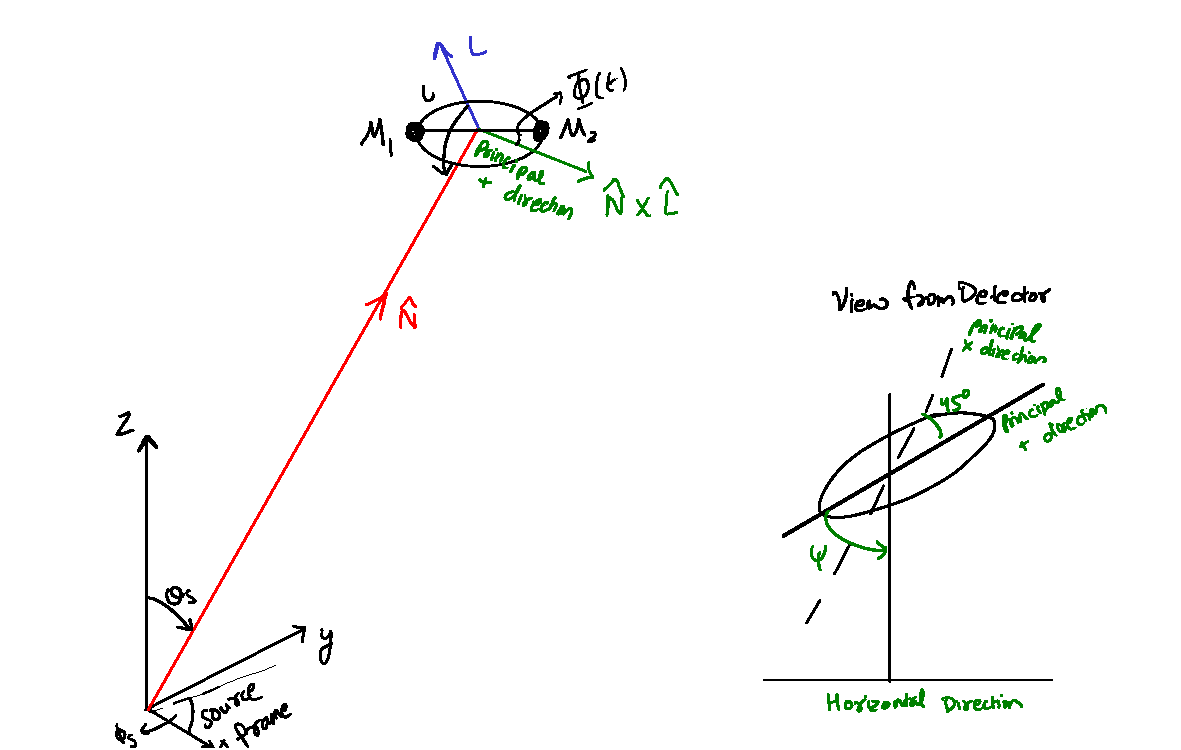
\includegraphics[scale=0.6]{../Figures/directions.pdf}
\caption{The definitions of various directions used in the equations. Left figure shows how the binary projected on the sky looks like.\label{fig:directions}}
\end{figure}

\begin{figure}[ht]
\centering
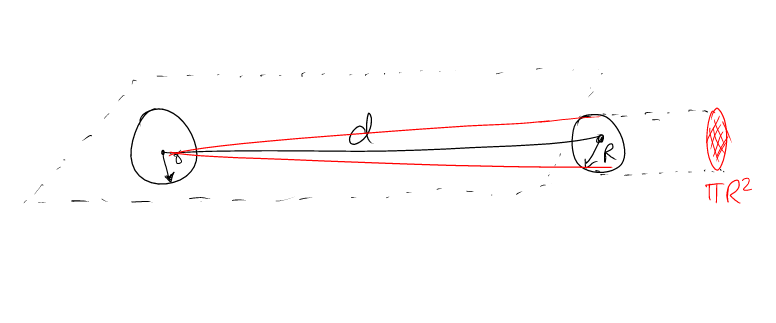
\includegraphics[scale=0.5]{diagram1.png}
\label{1}
\caption{The binary system HP Lib}
\end{figure}

